\documentclass[letterpaper,12pt]{article}
\usepackage[utf8]{inputenc}
\usepackage{amsmath, amsfonts}
\usepackage[x11names]{xcolor}
\usepackage{pgfplots}
\usepackage{tikz}
\usepackage{braket}

\usetikzlibrary{arrows.meta}
\pgfplotsset{
  compat = newest,
  blank_style/.style={
    clip=false,
    width=5cm,height=5cm,
    axis equal,
    axis line style={draw=none},
    tick style={draw=none},
    ticks=none,
    line width=1pt,
  },
}

% remove spacing around date and author
\usepackage{titling}
\predate{}
\postdate{}
\preauthor{}
\postauthor{}

\author{}
\title{MATH 262 - Homework 7.1}
\date{} % clear date

\begin{document}

\maketitle

\begin{enumerate}
  \item[8.]
    Arguing geometrically, find all eigenvectors and eigenvalues of the linear transformation below. Then find an eigenbasis if you can, and thus determine whether the given transformation is diagonalizable.
    \begin{center}
      The linear transformation with $T(\vec{v}) = \vec{v}$ and $T(\vec{w}) = \vec{v} + \vec{w}$ for the vectors $\vec{v}$ and $\vec{w}$ in $\mathbb{R}^2$ sketched below.
    \end{center}
    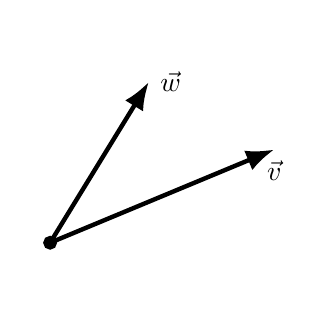
\begin{tikzpicture}
      \begin{axis}[blank_style]
        \addplot[black, mark=*] coordinates {(0, 0)};

        \addplot[-Latex, black, ultra thick] coordinates {
          (0, 0)
          (202, 84)
        } node[below,pos=1] {$\vec{v}$};

        \addplot[-Latex, black, ultra thick] coordinates {
          (0, 0)
          (89, 145)
        } node[right,pos=1] {$\vec{w}$};
      \end{axis}
    \end{tikzpicture} \\
    The definition of an eigenvalue states that it is a $\lambda$ such that $A\vec{u} = \lambda\vec{u}$. For $T(\vec{w})$, this would mean $\vec{v} + \vec{w}$ has to be a scalar multiple of $\vec{w}$. Thus, $\vec{v}$ would have to be collinear with $\vec{w}$. However, the sketch above shows that they are not collinear. As further proof, the sketch below illustrates $T(\vec{w})$. Observe that it is not collinear with $\vec{w}$. \\
    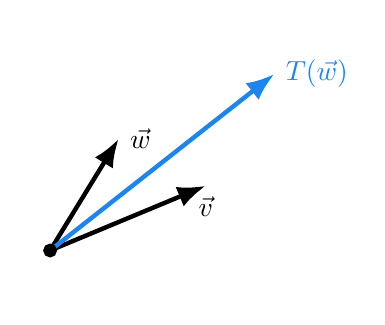
\begin{tikzpicture}
      \begin{axis}[blank_style]
        \addplot[black, mark=*] coordinates {(0, 0)};

        \addplot[-Latex, black, ultra thick] coordinates {
          (0, 0)
          (202, 84)
        } node[below,pos=1] {$\vec{v}$};

        \addplot[-Latex, black, ultra thick] coordinates {
          (0, 0)
          (89, 145)
        } node[right,pos=1] {$\vec{w}$};

        \addplot[-Latex, DodgerBlue2, ultra thick] coordinates {
          (0, 0)
          (291, 229)
        } node[right,pos=1] {$T(\vec{w})$};
      \end{axis}
    \end{tikzpicture} \\
    Therefore, $T$ is not diagonalizable.
\end{enumerate}

\end{document}
